\section{Background}\label{chap:background}

Here, the general concepts and techniques used in this work will be presented, in order to guide the reader in a way that he clearly understands what will be addressed in the following chapters.

\subsection{Natural Language Processing}

Natural Language Processing or NLP is a field whose purpose is to make computers perform tasks using human languages, such as allowing human-machine communication or performing useful processing over text or speech. Within this area, we have an example, \textbf{dialogue systems} or \textbf{conversational agents} used by chatbots these days. They try to imitate a natural conversation with humans. In these systems, a series of components must be studied as \textbf{speech recognition}, \textbf{natural language understanding}, and \textbf{speech synthesis}. Another important task in NLP is \textbf{question answering} that tries to give answers to the search for the users which can be in the form of textual or spoken questions. Currently, these searches can already be answered by web search engines, while they are not yet able to relate multiple sources of information by summarizing or making inferences between them. Currently, these systems use a series of components such as \textbf{information extraction} (IE), \textbf{word sense disambiguation}, and so on. \cite{Jurafsky:2009:SLP:1214993}.

According to \citetexto[p.~29]{Jurafsky:2009:SLP:1214993}, "What distinguishes language processing applications from other data processing systems is their use of \textit{\textbf{knowledge of language}}.". That is, for several NLP activities you need knowledge about phonetics, phonology, morphology, lexical semantics, compositional semantics. \cite{Jurafsky:2009:SLP:1214993}.


\subsection{Synonym}

According to \citetexto[p.~89]{zgusta1971manual}, "[...]synonyms: they are words which have different forms but identical meaning.". So we can say that synonyms can be defined as expressions with the same meaning. The definition we find in dictionaries like synonyms usually refers generally to any of the different types of synonyms, being near-synonyms and absolute-synonyms. \textbf{Near-synonyms} can be defined as expressions that are more or less similar, but not identical in meaning. Common examples in English are ’mist’ and ’fog’ or ’buy’ and ’purchase’. \textbf{Absolute synonyms} are one or more words whose meaning is identical and can be used with the same connotation in all different contexts and are equivalently semantic.  Therefore, they are extremely rare. \cite{lyons1995linguistic}.

\subsection{Hyponyms and hypernyms}

Hyponym can be defined by the lexical relation corresponding to the insertion of one class into another. That is, it shows the relation between a generic term and a specific instance of it, where the most specific term is the Hyponym and the generic class is Hypernym. So if we say that purple is a kind of color, then purple is a hyponym of color and color is the hypernym of purple. Because of this Hypernym is normally referred to as the \textit{is-a} and \textit{is-a-kind-of} relation. \cite[p.~88]{cruse1986lexical}.

\subsection{Lexical knowledge base - WordNet}

WordNet is one of the lexical resources most used over the last few years when it comes to word senses. \cite{fellbaum1998}. It is a large lexical database of English which consists of four sub-nets, one each for nouns, verbs, adjectives, and adverbs. Each of this has a set of lemmas annotated with a set of synonyms. WordNet can either be downloaded for free or accessed via the web. \cite{wordnetOnline2010}.

When searching for a word in this database, we will get a list of senses, where for each one we have a set of synonyms (also called \textbf{synsets}) and a brief description (gloss) and also sometimes a simple example of use. One of the most important relations of WordNet is the set of near-synonyms for a sense called synset. For example, when searching for 'car' we get the words auto, automobile, machine and motorcar for one specific sense. Also, all these senses are linked with others forming a network. One of the most common links between synsets is the hypernym, hyponymy. With this, each synset is linked with more generic synsets through its hypernym relation and also to more specific synsets through its hyponymy relation. There's also a way to distinguish words between nouns and instances like specific persons, countries and geographic entities.

There are some algorithms that can be used to find similar synsets in WordNet.

\begin{itemize}
    \item \textbf{Path Distance Similarity}: It is a scaled metric for measuring the similarity between a pair of senses based on the shortest path that connects the senses in the hypernym/hyponym taxonomy. \cite{meng2014measuring}.
    \item \textbf{Wu-Palmer Similarity}: Based on the depth of the senses in the taxonomy and of their Least Common Subsumer (most specific ancestor node). \cite{meng2014measuring}.
\end{itemize}

\subsection{Word embedding}

Word embeddings or vector space models of word semantics can be seen as a way of representing words, allowing the creation of NLP applications capable of understanding textual analogies even with few data for training. They are widely used for NLP in the last years.

% https://arxiv.org/abs/1708.02709

In many traditional NLP applications, \textbf{one-hot vectors} were used to represent words of a vocabulary. In this case, we have a vector for each word of the vocabulary with the same size, filled with zeros beside the position of the word where we have the value one. 
One problem of using the one-hot representation is that you can't generalize crosswords because of the inner product of any 1-hot vector is always zero. And for this reason, we cannot apply any distance-like metrics to evaluate the similarity. For this reason, a \textbf{feature vector} is preferable to word representation. In this case, we have for each word an vector of size $d$ filled with real values between 0 and 1 that represents multiple features. There are several ways to learn these high dimensional feature vectors values. 

These feature vectors or embeddings can be generated using neural networks. \citetexto{Bengio:2003} first introduced the term word embeddings with a simple feed forward neural language model to learn these vectors. After this, other models emerged with the creation of a toolkit named \textit{word2vec} presented by \citetexto{Mikolov2013DistributedRO}.

\textbf{Word2vec} is a predictive embedding model composed by two main architectures to produce word embeddings, as shown in \autoref{fig:word2vec}:

\begin{itemize}
    \item \textbf{Continuous bag-of-words} (CBOW): Learns the embedding by predicting the current word based on their surrounding words (context).
    \item \textbf{Skip-gram} (SG): It is the opposite of CBOW, it learns by predicting the surrounding words (context) given a current word.
\end{itemize}

\begin{figure}[h]
	\caption{Word2Vec training architectures.}
	\label{fig:word2vec}
	\centering%
	\begin{minipage}{.9\textwidth}
		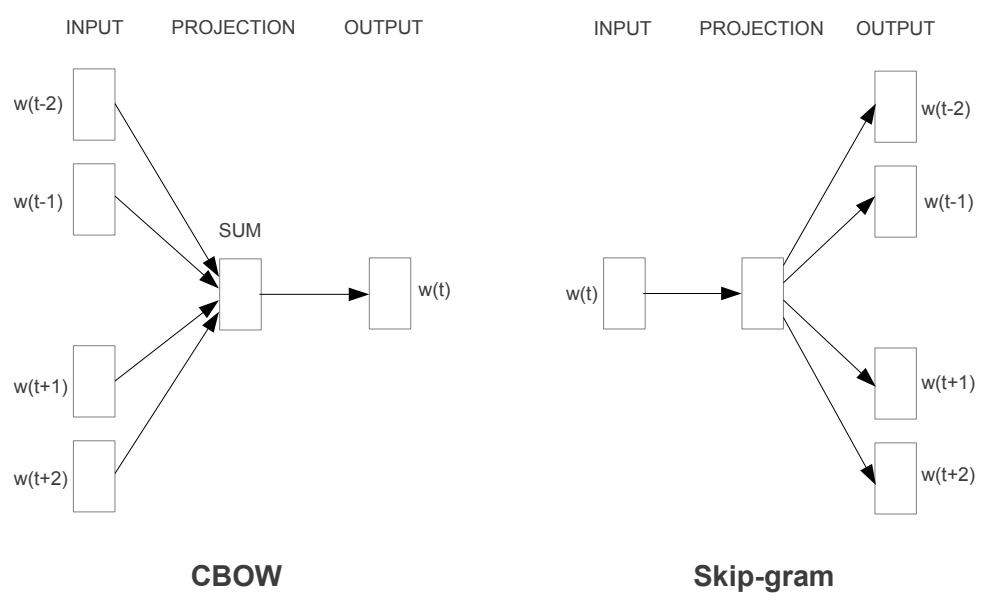
\includegraphics[width=\textwidth]{word2vec.png}
		\fonte{Taken from \citetexto[p.~5]{DBLP:journals/corr/abs-1301-3781}.}
	\end{minipage}
\end{figure}

After word2vec other algorithms emerged, such as \textbf{Global Vectors} (GloVe). \citetexto{Pennington2014} describes their work as "GloVe, is a new global log-bilinear regression model for the unsupervised learning of word representations that outperforms other models on word analogy, word similarity, and named entity recognition tasks.". GloVe is an approach that combines the global statistics of matrix factorization with the context based learning from word2vec.

\citetexto{Ling:2015:naacl} presents \textbf{Wang2vec} an extensions of the original word2vec models to improve the embeddings obtained for syntactically motivated tasks, by introducing changes that made the network aware of the relative positioning of context words.

Later on, \citetexto{bojanowski2016enriching} introduces \textbf{FastText}, which is another way to learn word representations by taking into account subword information. They incorporate character $n$-grams into the Skip-Gram model. By their evaluation the model outperforms baselines that do not take into account subword information.

% --------------------------

% The other family of word embedding model learns semantics by passing a window over the corpus line-by-line and learning to predict either the surroundings of a given word (Skip-gram model), or predict a word given its surroundings (continuous bag-of-words model). Note the bag-of-words problem is often shortened to “CBOW”.

% According to Mikolov et at., the authors of the word2vec paper, the two approaches differ slightly in performance:

% Skip-gram: works well with small amount of the training data, represents well even rare words or phrases.
% CBOW: several times faster to train than the skip-gram, slightly better accuracy for the frequent words.
% The authors of the GloVe paper note, however, that these context window-based methods suffer from the disadvantage of not learning from the global corpus statistics. As a result, repetition and large-scale patterns may not be learned as well with these models as they are with global matrix factorization. 

\subsection{Word similarity}

We can think of synonyms as a way to determine if two words are similar or not. In other words, they are similar if they have the same meaning, or are near-synonyms. According to \citetexto[p.~749]{Jurafsky:2009:SLP:1214993},

\begin{quote}
Two words are more similar if they share more features of meaning, or are near-synonyms. Two words are less similar, or have greater semantic distance, if they have fewer common meaning elements. Although we have described them as relations between words, synonymy, similarity, and distance are actually relations between word senses. For example of the two senses of bank, we might say that the financial sense is similar to one of the senses of fund while the riparian sense is more similar to one of the senses of slope.
\end{quote}

% According to \citetexto[p.~204]{Hatzlvassiloglou1999DetectingTS},
% \begin{quote}
% Similarity is a complex concept which has been widely discussed in the linguistic, philosophical, and information theory communities. For example, Frawley [1992] discusses all semantic typing in terms of two mechanisms: the detection of similarity and difference. Jackendoff [1983] argues that standard semantic relations such as synonymy, paraphrase, redundancy, and entailment all result from judgments of likeness whereas antonymy, contradiction, and inconsistency derive from judgments of difference. Losee [1998] reviews notions of similarity and their impact on information retrieval techniques.
% \end{quote}

The ability to identify the semantic similarity between words has been a subject of research very explored in the last years, because it is related to a series of activities of the area of natural language processing like information retrieval, text summarization, categorization and generation, database schema matching, question answering, machine translation, and others. \cite{Islam2007ApplicationsOC, Jurafsky:2009:SLP:1214993}. 

In short, the techniques for identifying similarity can be classified into two main approaches, knowledge-based and distributional-based. \textbf{Knowledge-based} similarity models are those that rely on pre-existing knowledge resources, such as thesauri, semantic networks, taxonomies, or encyclopedias. \cite{Agirre2009}. Moreover, almost all techniques concerning the \textbf{distributional-based} approach come from the basis of statistical semantics in which we have the Distribution Hypothesis which is defined by the fact that words occurring in the same contexts tend to have similar meanings. \cite{Harris1954}. Here the techniques are formed mainly by inducing distributional properties of words from corpora. \cite{Agirre2009}.


